\documentclass[a4paper,11pt]{article}
%\documentclass[a4paper,10pt]{scrartcl}

\usepackage[utf8]{inputenc}
\usepackage[a4paper,
            bindingoffset=0.2in,
            left=1in,
            right=1in,
            top=1in,
            bottom=1in,
            footskip=.25in]{geometry}
\usepackage{graphicx}
\usepackage{amsmath}
\usepackage{float}
\usepackage{tabu}
\usepackage{xcolor}
\usepackage{fancyhdr}
\usepackage{hyperref}
\usepackage{enumitem}
\setlist{nosep}
\hypersetup{
    colorlinks=true,
    linkcolor=blue,
    filecolor=magenta,      
    urlcolor=cyan
    }
\usepackage{tocloft}
\renewcommand{\cftsecleader}{\cftdotfill{\cftdotsep}}
\usepackage{titling}
\renewcommand\maketitlehooka{\null\mbox{}\vfill}
\renewcommand\maketitlehookd{\vfill\null}
\usepackage{parskip}
\graphicspath{{../figures/}}

\title{Using Autoencoders to Detect Errors in Telemetry Events}
\author{Andrew Younger}
\date{\today}

\begin{document}
\pagenumbering{gobble}
\begin{titlingpage}
 \maketitle
\end{titlingpage}
%\newpage
%\pagenumbering{roman}
%\tableofcontents
\newpage
\pagenumbering{arabic}
\section{Introduction}
Telemetry events are essential for accurate reporting on player activity and progress for modern games. They allow the analytics team to dive deeply into topics and analyze important questions from stakeholders in the project. These events can be quite expansive, detailing anything from how a player kills an enemy to what cosmetics a player applies to their character to how quickly players are able to complete the game.
\par
During the development cycle of a game there are frequent code changes which can affect telemetry frequently both accidentally and by design. QC teams work diligently in order to keep up with testing events as they are created but changes that affect older events often produce bugs which impact reporting done by the analytics team for playtests. In addition, telemetry events can be quite large and have many attributes with many different possibilities. A player.kill event, for example, where there are 50 weapons and 50 enemy types tracked yiels 2500 possibilities in just two columns. This further exacerbates the issues that the QC teams face when trying to catch every erroneous scenario that occurs inside telemetry events leading to the questions of: ``How do we determine when an event has bugs?'' and ``How do we know when QC teams should retest old events?''.
\par
An immediate proposition to answer these questions is to use some form of automated bug detection. There are two methods of bug detection which could be helpful for QC teams to track down and deal with bugs: checking for some sort of spike in event frequency (if events start transmitting too often or stop transmitting then there may be an issue with the event's trigger mechanism) and statistsically determining if event attribute A is supposed to match with event attribute B. This report outlines a process for the second method by using an autoencoder to learn the possibility space of an event.
\subsection{Autoencoders}
Autoencoders are type of neural network that fall into the \textit{encoder-decoder} family of neural networks. The general process for an autoencoder is shown in Figure \ref{autoencoder_general}. The encoding section of an autoencoder learns to ``compress'' the data down into a smaller dimension so that the decoding section of the autoencoder can attempt to recreate the original data from this low-level representation of the data. Autoencoders are used for several purposes including: image denoising, facial recognition, and, importantly for finding bugs, anomaly detection.
\begin{figure}[H]
\centering
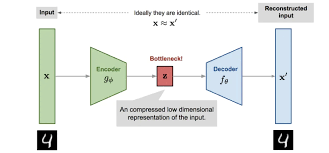
\includegraphics[width=.8\textwidth]{autoencoder_general.png}
\caption{The general layout of an autoencoder network. The network works by learning efficient compression to a low dimension and then reconstructing the data as closely as possible.}
\label{autoencoder_general}
\end{figure}
Using an autoencoder to detect anomalies in data is done by looking for data entries that have too high of an error in reconstruction. The error function is generally mean squared error (MSE) or mean average error (MAE). A threshold can be set, either manually or using some statistical methods, and any entry that gives a higher reconstruction error than the threshold is flagged as an anomalous event. For this particular scenario autoencoders are a prudent choice because they learn the specific data they were trained on quite well which leads to a much larger reconstruction error for anomalous entries. Telemetry events correspond to specific actions in-game and as such the majority of events should not be anomalies which gives autoencoders a larger advantage - especially when combined with semi-supervised learning methods.
\subsection{Semi-Supervised Learning}
Machine learning problems are often considered to fall into the either the category of supervised learning or into unsupervised learning. Semi-supervised learning provides a middle ground between the two methods where a model can be sufficiently trained on a dataset where only a small percentage of data points are labeled as anomalies beforehand. Under the assumption that \textit{most} of the data entries are not anomalies a semi-supervised autoencoder can be trained to detect erroneous entries.
\section{Methods and Models}
In order to determine if a semi-supervised autoencoder is a suitable candidate for detecting bugs in telemetry events multiple experimental steps were taken:
\begin{enumerate}
 \item Proof of concept model using a specific bug that was found and fixed as well as the fixed events corresponding to the expected behaviour of the event.
 \item The same bug and corrected behaviour but testing MSE as the error function instead of MAE.
 \item A larger-scale version of the initial proof of concept that has a smaller percentage of known anomalies.
 \item A model that is truly semi-supervised and uses a large number of arbitrary events to detect the specific bug.
\end{enumerate}
Many telemetry events are designed to give context on what tools a player is using and how the player uses them and thus many of the most important attributes of a telemetry event are categorical data. To have a model read categorical data it must be ``translated'' into some numerical form. 
\subsection{One-Hot Encoding}
One-hot encoding is a common method to do this and works by turning each categorical entry in a column of distinct length $n$ into a sparse vector of length $n$ where only the corresponding entry is non-zero. For an example of how this process works consider a simple dataset where each entry is simply an ID column, a colour and a shape:
\begin{center}
\begin{tabular}{ |c|c|c| } 
 \hline
 ID & Colour & Shape \\ \hline
 1 & Blue & Square \\
 2 & Red & Triangle \\
 3 & Red & Square \\
 4 & Orange & Circle \\
 5 & Pink & Circle \\
 \hline
\end{tabular}
\end{center}
To use one-hot encoding and vectorize this dataset first look at the number of unique entries in each categorical field. There are 4 unique colours and 3 unique shapes so each entry in the colour column will be a sparse vector of length 4 and each entry in the shape column will be a sparse vector of length 3. The vectorized  entries would look like this:
\begin{center}
\begin{tabular}{ |c|c|c| } 
 \hline
 ID & Colour & Shape \\ \hline
 1 & [1 0 0 0] & [1 0 0] \\
 2 & [0 1 0 0] & [0 1 0] \\
 3 & [0 1 0 0] & [1 0 0] \\
 4 & [0 0 1 0] & [0 0 1] \\
 5 & [0 0 0 1] & [0 0 1] \\
 \hline
\end{tabular}
\end{center}
Each entry in the vector can be thought of as a binary flag for the entry: ``Is it blue? Is it red?'' etc. All the different models that were trained used one-hot encoding as part of the data preprocessing.
\subsection{Proof of Concept Model}
The original proof of concept model used a relatively small size of proper telemetry events and a relatively high number of anomalous events to compare against. The dataset that was chosen for the original proof of concept model was from Watch Dogs: Legion and used the player.kill event. This model was trained against a specific bug that was found and fixed; when players destroyed an enemy drone it would occasionally register as a melee kill even when the player had used a gun to destroy the drone. Ten thousand player.kill events where a drone was destroyed and sent a proper event were used and one thousand of the aforementioned bugged events were used.
\par
The training and testing process for this model was replicated for the subsequent models that were created.
\begin{enumerate}
 \item Split data into train/test sizes. 80\% training size was used.
 \item Normalize numerical data columns.
 \item Vectorize categorical columns using one-hot encoding.
 \item Train the autoencoder on the processed data.
 \item Determine a threshold for what constitutes an anomalous event.
\end{enumerate}
There are a few options for determining the threshold for anomalous events. The first is to look at the reconstruction errors and manually pick a threshold that separates the proper events from the anomalies. This could lead to a lot of inconsistency in other use-cases so in order to have a consistent threshold it was chosen to be one standard deviation away from the mean reconstruction error. For this first model this was a threshold of 0.708. Any reconstruction error above this was labeled as a bugged event. Figure \ref{original_poc_training_reconstruction} shows the reconstruction errors for the training of the model.
\begin{figure}[H]
\centering
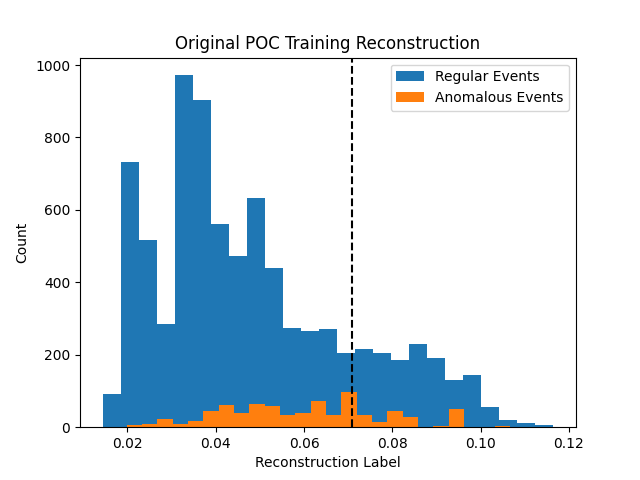
\includegraphics[width=.8\textwidth]{original_poc_training_reconstruction.png}
\caption{Reconstruction errors for regular events and anomalous events during training. The black line shows the anomaly threshold.}
\label{original_poc_training_reconstruction}
\end{figure}
During training it is easy to see that the majority of regular events have a reconstruction error that is less than the calculated threshold. However many of the known anomalous events are also lower than the calculated threshold. There is even a higher percentage of the regular events that are higher than the threshold than there are anomalous events. This ultimately led to a relatively low accuracy score for the original proof of concept. The scores for the original model are shown in the table below. With the exception of the model accuracy the metrics are very promising for a proof of concept. In Figure \ref{original_poc_test} the testing reconstruction errors can be seen and the reconstruction errors for only anomalous events can be seen in Figure \ref{original_poc_anomaly}.
\begin{center}
\begin{tabular}{ |c|c| } 
 \hline
 Metric & Score \\ \hline
 Accuracy & 78\% \\
 Precision & 91\% \\
 Recall & 84\% \\
 F1 Score & 87\% \\
 \hline
\end{tabular}
\end{center}
\begin{figure}[H]
\centering
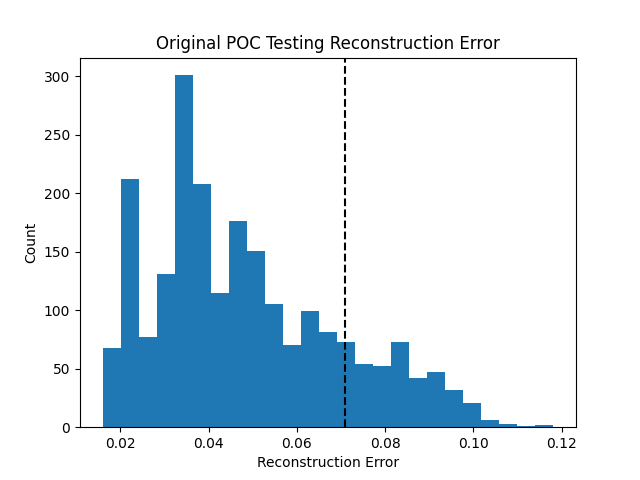
\includegraphics[width=.8\textwidth]{original_poc_test_reconstruction.png}
\caption{Reconstruction errors for regular events and anomalous events during testing. The black line shows the anomaly threshold.}
\label{original_poc_test}
\end{figure}
\begin{figure}[H]
\centering
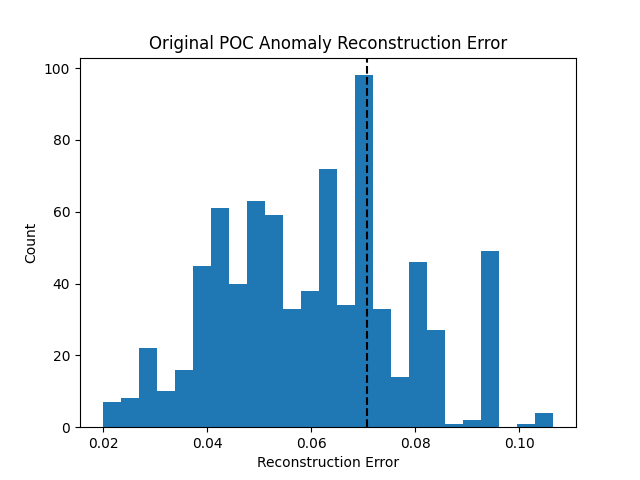
\includegraphics[width=.8\textwidth]{original_poc_anomaly_reconstruction.png}
\caption{Reconstruction errors for regular events and anomalous events during testing. The black line shows the anomaly threshold.}
\label{original_poc_anomaly}
\end{figure}
From these two graphs it is easier to see that the model was very good at identifying anomalous events after training finished. The immediate concern is the how low the accuracy and the recall for the model are. This could be the result of the relatively high number of anomalous events. Almost 10\% of the training data was anomalous and in a realistic scenario bugs likely between 2\% and 3\% of events at most. In a future model this percentage is lowered to a more realistic amount.
\subsection{MSE Model}
The second model was identical to the first in both data and process with the only exception that the error function was switched from MAE to MSE. Since MSE uses the square of the error instead of the average it should give a higher relative error for the anomalies. The MSE model improved all the metrics but only very slightly - less than 1\%. However any improvement is good and so MSE is the chosen error function for futre models.
\subsection{Small Sample Model}
The small sample model is very similar to the original proof of concept. The main difference is that the ratio of regular events to labeled anomalous events is much smaller. Instead of ten thousand regular events and one thousand anomalies it used thirty thousand regular events and the same one thousand anomalies.
                                                                                                                                

%\newpage
%\begin{thebibliography}{100}
%\bibitem{patil} Akshay Gadi Patil, Omri Ben-Eliezer, Or Perel, and Hadar Averbuch-%Elor, ``Recursive Autoencoders for Document Layout Generation'' {\tt arXiv:%1909.00302v4 [cs.CV]}
%\end{thebibliography}

\end{document}
